\section{Dielectric Simulations}

Sharp edges, corners or triple points of dielectric and conductive bodies are typical field enhancement regions. \newline
\begin{minipage}[lt]{15cm}
	Following arrangements can limit these enhancements:
	\begin{itemize}
		\item Geometrical rounding of the sharp corners and edges reduces the electric field around them and thus mitigate the dielectric problems.
		\item Shielding, where the shield is on the same potential.
		\item Coating with a high(er) permittivity material. 
		\begin{equation*}
			\vec{D_2}\cdot \vec{n} = \vec{D_1}\cdot \vec{n} \Rightarrow E_{n,\textrm{2}} = \frac{\varepsilon_{r1}}{\varepsilon_{r2}} \cdot E_{n,\textrm{1}}
		\end{equation*}
		\begin{equation*}
			V = E_2 \cdot d_2 + E_1 \cdot d_1 \Rightarrow E_2 = \frac{V}{d_1\cdot \frac{\varepsilon_{r2}}{\varepsilon_{r1}}+d_2}
		\end{equation*}
		\item Hiding triple points to capture the electrons $\rightarrow$ free ions recombine.
	\end{itemize}
\end{minipage}
\begin{minipage}[rt]{4cm}
	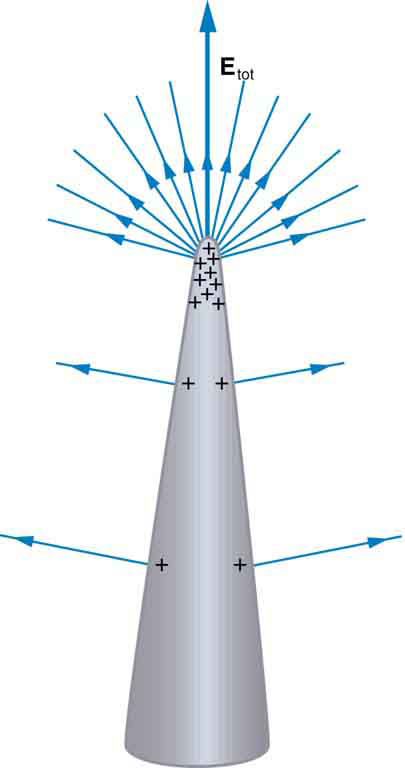
\includegraphics[width=.7\textwidth]{./images/fieldEnhancement.jpeg}
\end{minipage}
\\
\begin{minipage}{5cm}
	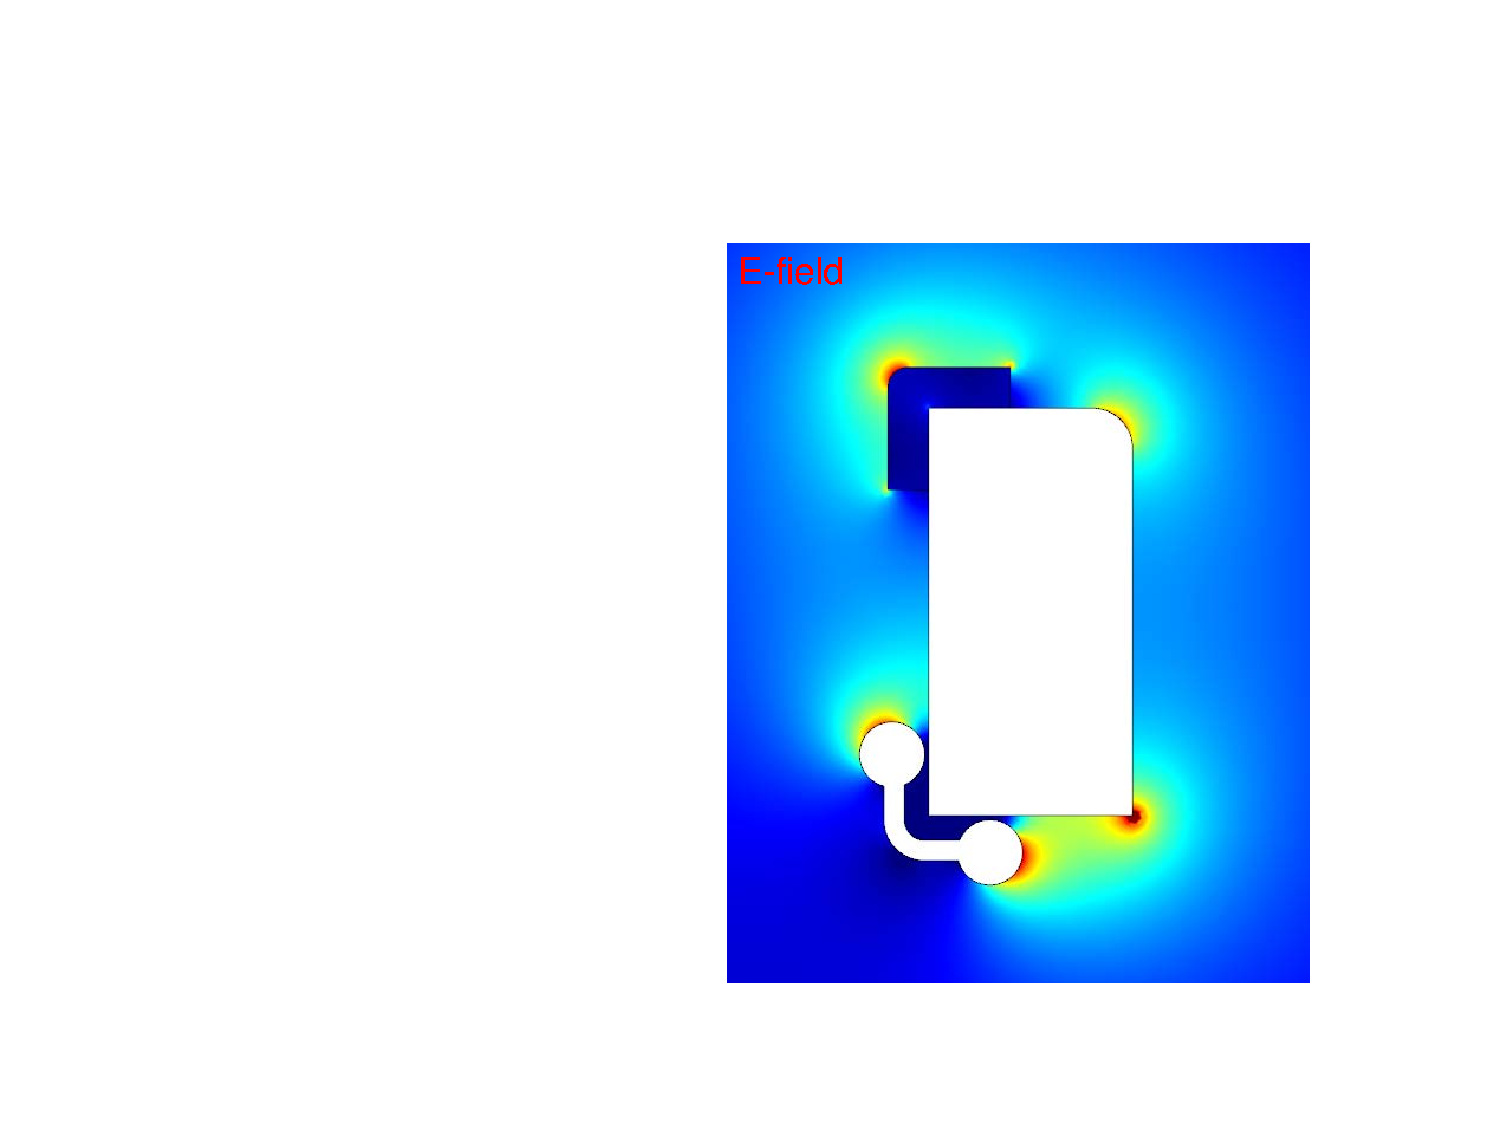
\includegraphics[width=.8\textwidth]{./images/EFields.pdf}
\end{minipage}
\begin{minipage}{7cm}
	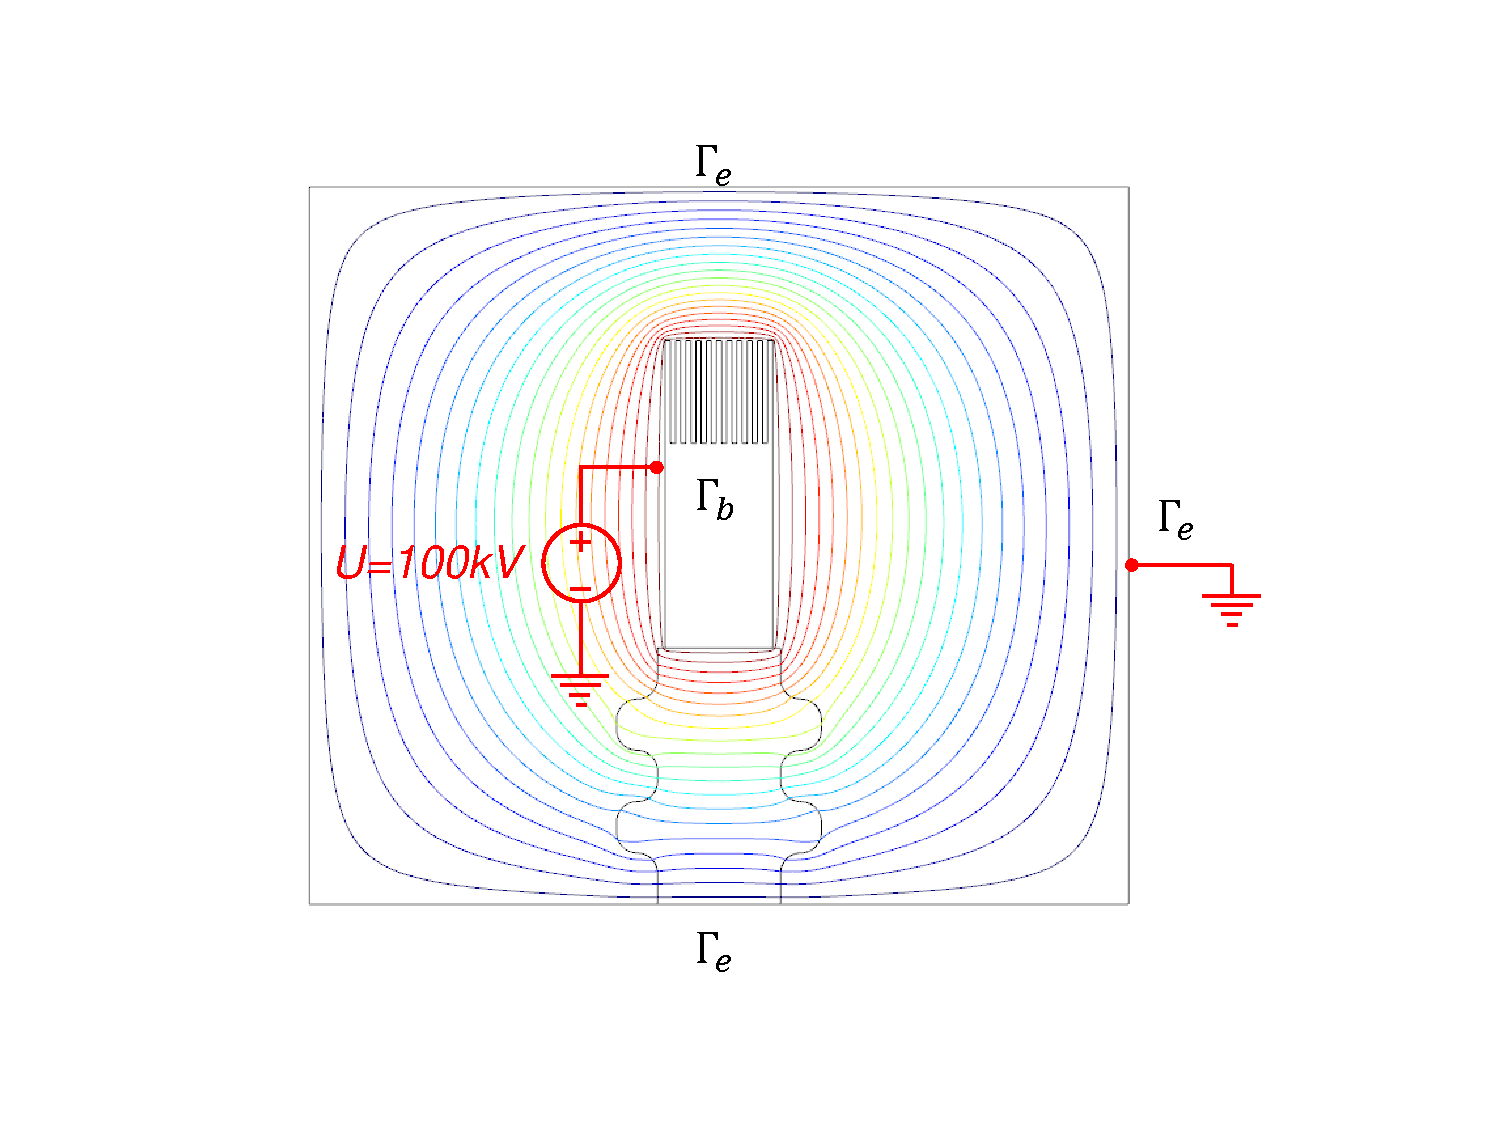
\includegraphics[width=.8\textwidth]{./images/Lines.pdf}
\end{minipage}
\begin{minipage}{7.5cm}
	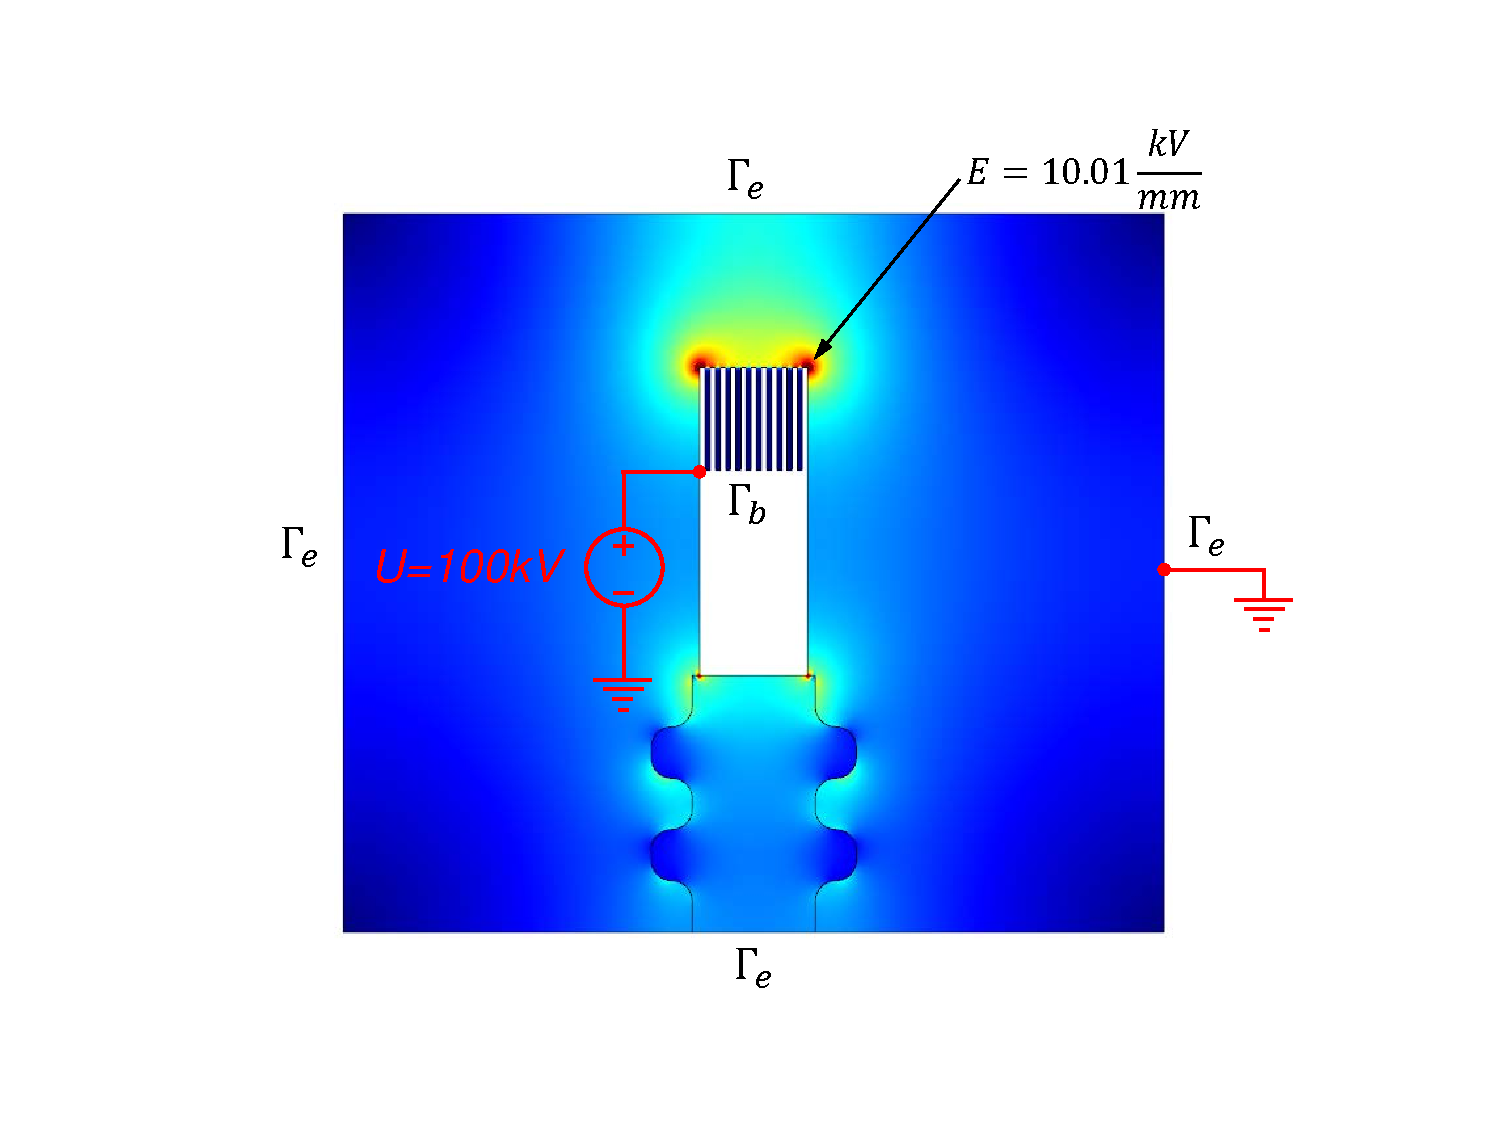
\includegraphics[width=.8\textwidth]{./images/Field.pdf}
\end{minipage}